\newcommand{\PLH}{H$^+$I\xspace}
\newcommand{\PLWH}{SH$^+$I\xspace}

%% START PROACT CHAPTER
\chapter{\proacttitle}
\label{chap:proact}
\clearpage

In \gls{HIV} epidemics, the majority of the structure of the transmission network is dictated by just a few individuals. Public health intervention, such as ensuring people living with \gls{HIV} adhere to \gls{ART} and are continually virally-suppressed, can help control the spread of the virus. However, such intervention requires utilizing the limited public health resource allocations. As a result, the ability to determine which individuals are most at-risk of transmitting \gls{HIV} could allow public health officials to focus their limited resources on these individuals. Molecular epidemiology suggests an approach: prioritizing people living with HIV based on patterns of transmission inferred from their sampled viral sequences. In this paper, we introduce ProACT (\textbf{Pr}i\textbf{o}ritization using \textbf{A}n\textbf{C}es\textbf{T}ral edge lengths), a novel phylogenetic approach for prioritizing individuals living with \gls{HIV}. ProACT uses a simple idea: ordering individuals by their terminal branch length in the phylogeny of their virus. In simulations and also on a dataset of \gls{HIV}-1 subtype B \textit{pol} sequences obtained in San Diego, we show that this simple strategy improves the effectiveness of prioritization compared to state-of-the-art methods that rely on monitoring the growth of transmission clusters defined based on genetic distance.

\section{Introduction}
The transmission of \gls{HIV} resembles scale-free networks~\cite{Wertheim2014}, in which the majority of the structure of the network is dictated by just a few individuals, a phenomenon likely resulting from the scale-free properties of sexual contacts and injection drug use along which \gls{HIV} is transmitted~\cite{Little2014,Schneeberger2004}. As a result, public health intervention may be more effective when targeted at people living with \gls{HIV} who are more likely to grow the transmission network. However, the best method to target individuals for specific interventions remains an open question, and the best strategy will likely depend on the specific intervention planned.

A potential form of intervention aiming to reduce future transmissions is to target \glspl{PLH}. For example, \gls{ART} suppresses the \gls{HIV} virus in the majority of cases, stops the progression of the disease, and prevents onward transmission to an uninfected sexual partner, provided the \gls{PLH} continuously adheres to the treatment~\cite{Cohen2011}. In addition to reducing risk of transmission at the molecular level, adherence to \gls{ART} is associated with a reduction of risky behavior as well~\cite{Bunnell2006}. While the initiation of \gls{ART} is routine (or even universal) in most advanced health care systems, not every case of \gls{ART} initiation leads to a sustained suppression of the virus through time. \glspl{PLH} who start \gls{ART} but fail to sustain it or who are otherwise unsuppressed can still infect others. Thus, a possible intervention is to ensure known \glspl{PLH} are kept on \gls{ART} and are continually suppressed, a task that requires allocation of public health resources. If people at risk of losing their suppression could be predicted accurately, the public health system could focus their limited resources on these individuals, administrating several types of interventions: followups to ensure sustenance of \gls{ART}, increased testing to ensure suppression, and, if all else fails, offering \gls{PrEP} to their sexual partners. However, these are all costly interventions and cannot be undertaken for every known \gls{PLH}. Thus, a natural question surfaces: which individuals are most at-risk of transmitting \gls{HIV}?

Predicting tendency for future transmissions is difficult and is fraught with danger if undertaken primarily based on demographic or behavioral traits. Molecular epidemics suggest an alternative method: prioritizing \glspl{PLH} for intervention solely based on patterns of transmission inferred from \gls{HIV} sequence data~\cite{Bbosa2019,Villandre2019,Oster2018,Ragonnet-Cronin2019,Wertheim2018,Wertheim2011,Wertheim2014,Smith2009}. The inference of transmission networks using phylogenetic or distance-based methods has been the subject of much research~\cite{Leitner2018,Pond2018,Ragonnet-Cronin2013,Prosperi2011}. However, in this work, instead of being concerned with inferring exact patterns of transmissions, we ask the following question: given molecular data from each \gls{PLWH}, presumably all with access to \gls{ART}, which individuals are most at-risk of transmitting the virus?

Prioritizing care based on molecular epidemics has been studied recently. Wertheim \textit{et al}. (2018) present a method for prioritizing \glspl{PLWH} based on performing transmission clustering (i.e., grouping individuals with low viral genetic distance into ``transmission clusters'') and ordering clusters  by growth rate~\cite{Wertheim2018}. On a large dataset from New York, they show that the approach is able to predict individuals who will have relatively larger numbers of transmission links in the near future. Moshiri \textit{et al}. (2018) have studied the same question in simulations and have shown that monitoring cluster growth can be used for predicting future transmissions substantially better than a random guess, whether clusters are defined using genetic distances or using phylogenetic methods~\cite{Moshiri2018}. Most recently, Balaban \textit{et al}. (2019) showed in simulations that using a cluster-monitoring approach similar to that of Wertheim \textit{et al}. (2018) but defining clusters  using a min-cut optimization problem gives a small but consistent improvement over defining clusters using genetic distances~\cite{Balaban2019}.

In this paper, we introduce a new method for ordering \glspl{PLWH} based  on their phylogenetic relationships. Instead of relying on clustering individuals and then ordering clusters based on their growth, we seek to order individuals without clustering and without reliance on parametric models. Instead, we seek to simply exploits patterns in the phylogeny, and in particular, in branch lengths.

\section{New Approaches}
ProACT (\textbf{Pr}i\textbf{o}ritization using \textbf{A}n\textbf{C}es\textbf{T}ral edge lengths) takes as input the inferred phylogenetic relationships between sampled \gls{HIV} viruses (e.g. from the \gls{pol} region), rooted using an outgroup or clock-based methods (e.g. midpoint or MinVar-root~\cite{Mai2017}). ProACT simply orders \glspl{PLWH} in order of incident branch length of their associated virus, and it breaks ties based on incident branch lengths of parent nodes, then those of grandparent nodes, etc. We first motivate the approach and then present a formal definition of the method.

We note that ProACT is motivated and tested in a context similar to the present day health care systems that enjoy enough resources to provide \gls{ART} to all \glspl{PLWH} (recall that we call a \gls{PLH} a \gls{PLWH} if their sequence is also sampled). Thus, each \gls{PLWH} is assumed to be given \gls{ART} at a time close to when their \gls{HIV} is sequenced, but they may fail to be suppressed for the remainder of their life. These conditions describe the common practice of care in many advanced and (increasingly) developing countries.

\begin{figure} % FIGURE 1 IN ORIGINAL PAPER
\centering
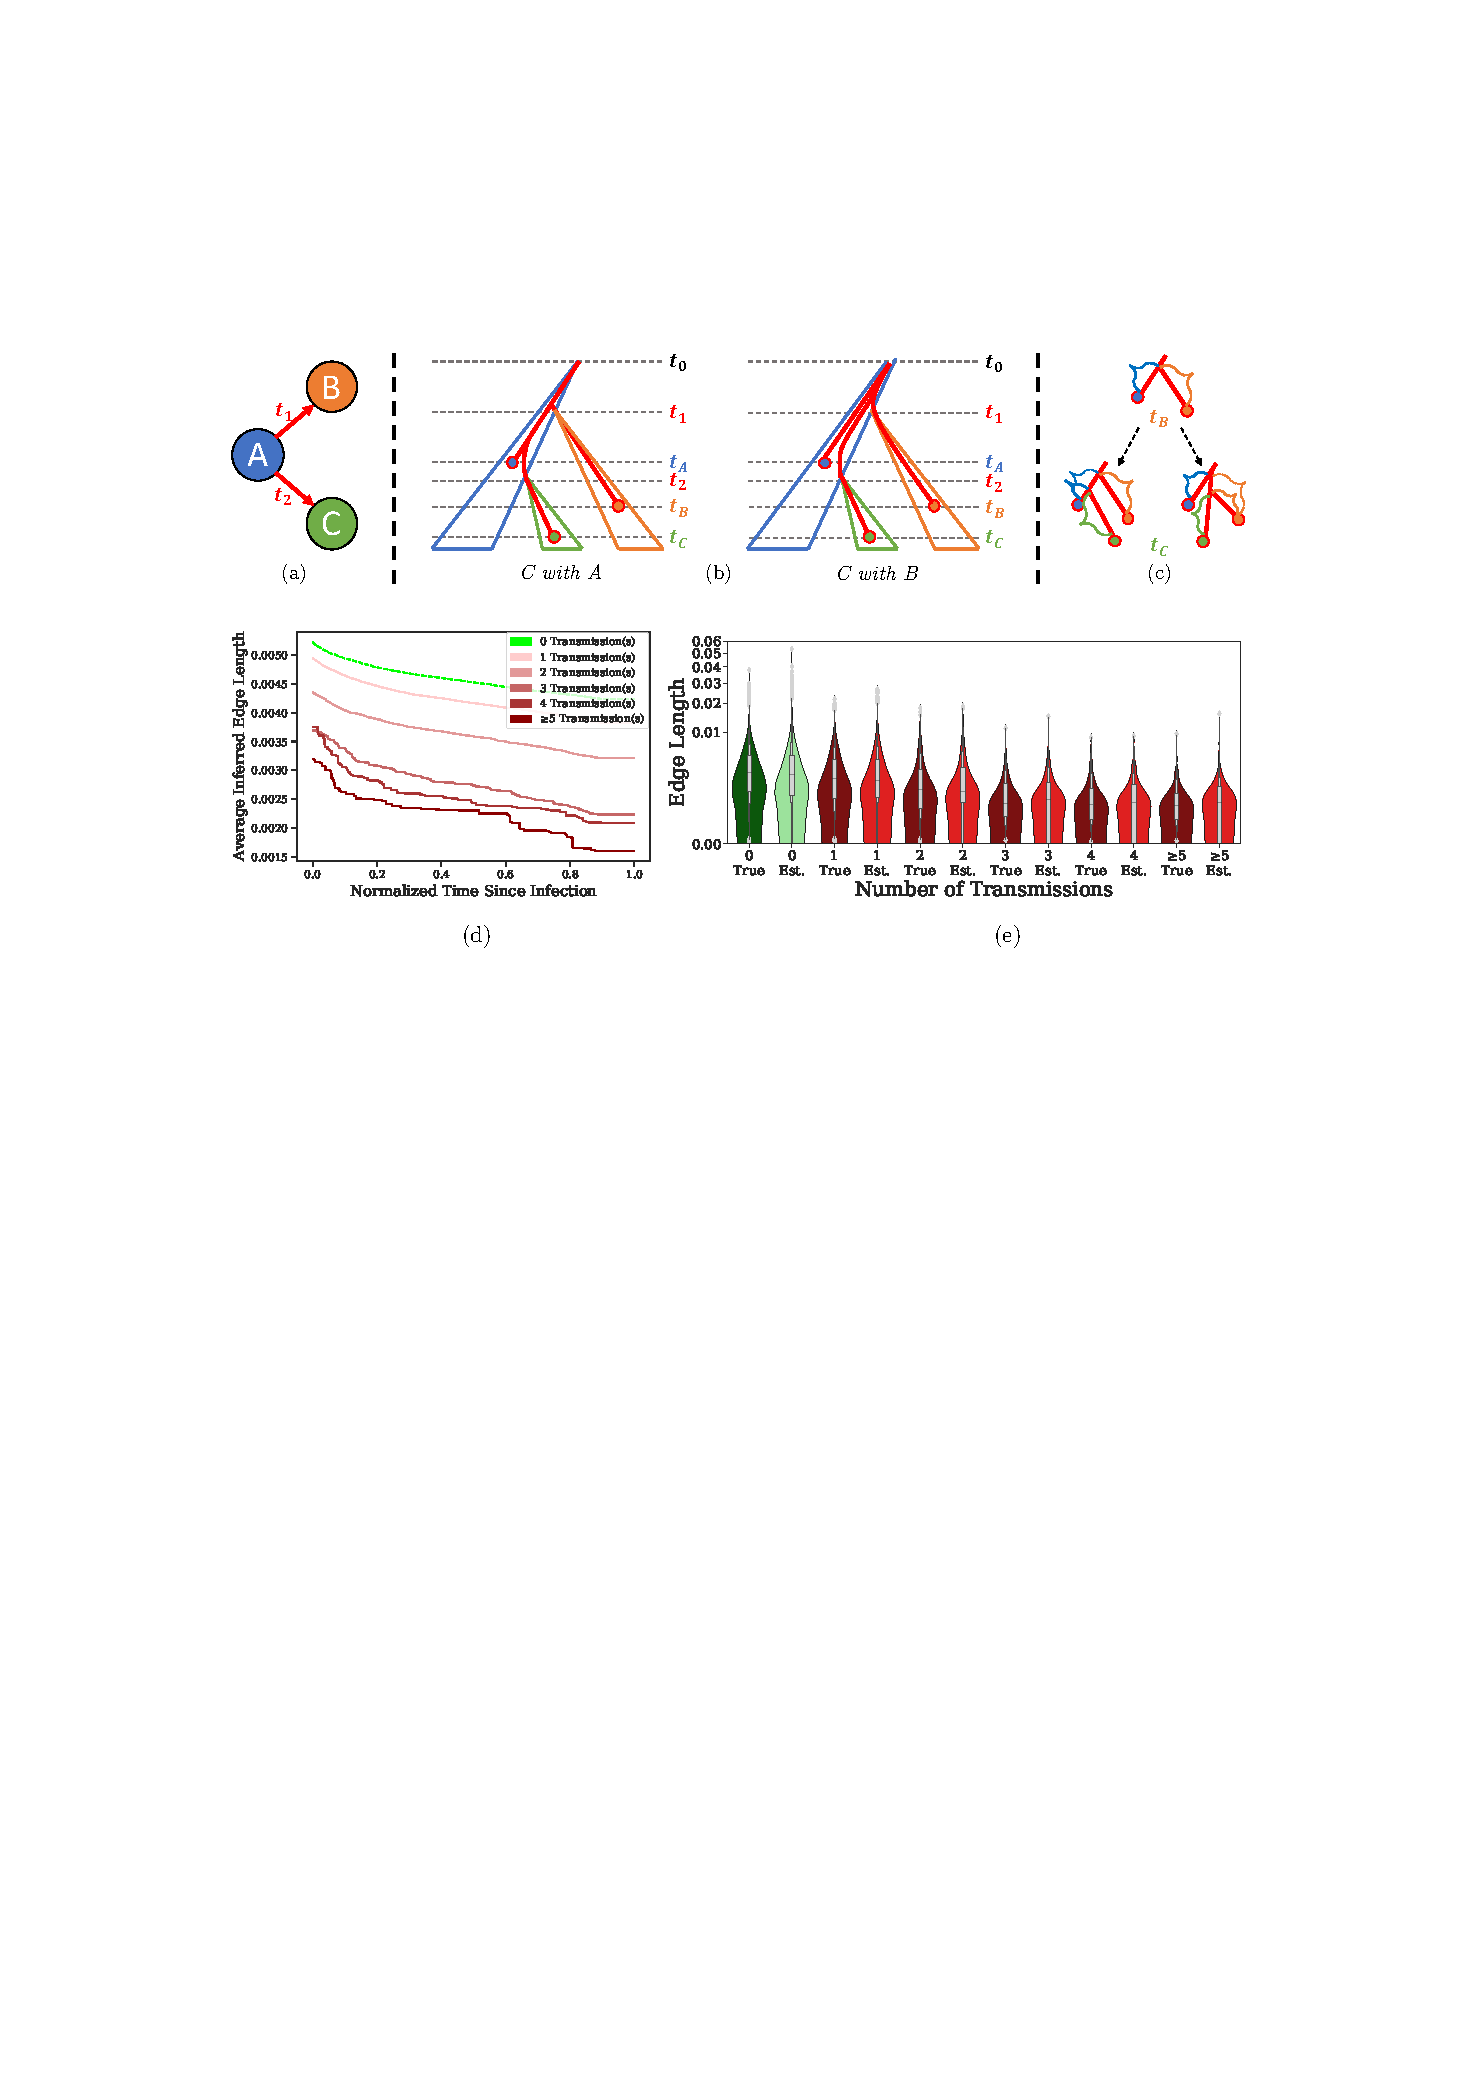
\includegraphics[width=\textwidth]{figs/proact-diagram}
\caption[ProACT Diagram]
{The effect of new transmissions on incident branch lengths. (a) Individual $A$ transmits to individual $B$ and $C$ at times at  $t_1$ and $t_2$, respectively. (b) Viral samples are obtained from individuals $A$, $B$, and $C$ at times $t_A$, $t_B$, and $t_C$. The viral phylogeny of samples is constrained by each transmission event's bottleneck, and the most likely phylogeny matches the transmission history (Left), but in the less likely deeper coalescence, it may not match (Right). (c) Moving from the phylogeny observed at time $t_B$ to the phylogeny at time $t_C$, the branch length incident to individual A  shortens upon the addition of individual C  in the likely event that the coalescence of the lineage from $C$ with the lineage from $A$ is more recent than its coalescence with the lineage from $B$ (Left), or the branch length incident to individual A remains constant in the event of a less likely deeper coalescence (Right). Regardless, the length of the branch incident to individual A never increases.
In simulation, we can observe this trend: as time progresses, the incident branch length of each individual tends to decrease, both in true (Fig.~\ref{fig:proact-true-bl-vs-time}) and inferred (d) phylogenies, and as the number of transmissions from a given individual increases, the distribution of incident edge length tends to decrease, both in true and inferred phylogenies, labeled ``True'' and ``Est.,'' respectively (e).}
\label{fig:proact-diagram}
\end{figure}

\subsection{Motivating the Approach}
We start with the observation that, in simulations (described in detail below), when a phylogeny is inferred from sequences obtained at a given time point in an epidemic,
the more a node transmits, the shorter its incident branch length tends to be (Figs.~\ref{fig:proact-diagram}d--e and~\ref{fig:proact-trans-vs-bl}). Using the Kendall's tau-b test~\cite{Kendall1938}, in a ten-year epidemic simulation (details described below), we found a statistically significant anticorrelation between the incident branch lengths of individuals sampled within the first 9 years of the epidemic and the number of individuals they infected over the final year of the epidemic. This held for true ($\tau=-0.0431$, $p\ll 10^{-10}$) and inferred ($\tau=-0.0354$, $p\ll 10^{-10}$) phylogenetic trees. Though not obvious, this observation can be explained by the constraints placed upon the viral phylogeny by the transmission history (Fig.~\ref{fig:proact-diagram}a--c).

In the context of \gls{HIV} epidemiology in many advanced countries, \glspl{PLWH} are typically sampled upon beginning \gls{ART}. Let's assume for simplicity that every individual in the given dataset has at some point initiated \gls{ART}, meaning future transmissions by individuals in the dataset must happen only if the source stops \gls{ART} or is otherwise unsuppressed. Given a viral phylogeny containing all known \glspl{PLWH}, if, in the future, individual $u$ in the dataset transmits to individual $v$, there are two possible scenarios regarding the placement of the leaf corresponding to $v$ in the existing (true) phylogeny: (1) $v$ is placed on the edge incident to $u$, so the edge incident to $u$ will shorten, or (2) $v$ is not placed on the edge incident to $u$, so the edge incident to $u$ will remain the same length. Although Scenario 2 is possible, Scenario 1 is far more likely \cite{Romero-Severson2016}, and note that the terminal branch lengths do not increase in either scenario. Thus, as time goes by, the terminal branch can only shorten or stay fixed, and it will most often shorten because of new transmissions by the \gls{PLWH} associated with that terminal branch. This pattern, easily observed in simulations (Fig.~\ref{fig:proact-diagram}d), leads to shorter branches for \glspl{PLWH} who have transmitted recently.

Note that \glspl{PLWH} who transmit are unsuppressed. The first time they infect others, their terminal branch length is likely to decrease, and further transmissions further decrease their terminal branch lengths (Fig.~\ref{fig:proact-diagram}d). Thus, one expects nodes with smaller incident branch length to be more likely to have transmitted since their sampling time. Moreover, they are also likely to transmit in the near future because they are likely not to be suppressed. The higher probability of a lack of suppression makes them a good candidate for intervention.

\subsection{Formal Description}
ProACT takes as input a \textit{rooted} phylogenetic tree $T$ of viral samples. Let $bl(u)$ denote the incident branch length of node $u$, and assume the incident branch length of the root of $T$ is 0. Let $a(u)$ denote the vector of ancestors of node $u$ (including $u$), where $a(u)_1$ is $u$, $a(u)_2$ is the parent of $u$, $a(u)_3$ is the grandparent of $u$, etc. Let $r(u)$ denote the length of the path from node $u$ to the root of $T$, i.e., $r(u)=\sum_{v\in a(u)}{bl(v)}$. ProACT sorts the leaves of $T$ in ascending order of $bl(a(u)_1)$, with ties broken by $bl(a(u)_2)$, then by $bl(a(u)_3)$, etc. Note that, for two leaves $u$ and $v$, $|a(u)|$ may be less than $|a(v)|$, in which case, for all $|a(u)|<i\le|a(v)|$, $\frac{r(u)}{|a(u)|-1}$ (i.e., average branch length along the path from $u$ to the root of $T$) is compared with $bl(a(v)_i)$ instead. If two nodes are equal in all comparisons, if the user provides sample times, the earlier sample time is given higher priority; otherwise, ties are broken arbitrarily. Because sorting is needed, for a tree with $n$ leaves, assuming branch lengths are fairly unique, the ProACT algorithm runs in $\bigO(n\log n)$ time. Scalable methods exist both for the inferring~\cite{Price2010,Nguyen2015} and rooting~\cite{Mai2017} very large trees.

\section{Results}
We evaluate ProACT on simulated and real data.

\begin{table}[!ht] % TABLE 1 IN ORIGINAL PAPER
\caption[Varied Simulation Parameters]{Varied \gls{HIV} simulation parameters. Values for the base model condition are shown in bold.}
\vspace{-0.25in}
\begin{center}
\begin{tabular}{|c|c|}
\hline
\textbf{Parameter} & \textbf{Values}\\
\hline
\gls{ART} Start Rate ($\lambda_+$, year$^{-1}$) & \textbf{1}, 2, 4\\
\hline
\gls{ART} Stop Rate ($\lambda_-$, year$^{-1}$) & 0.12 (0.25x), 0.24 (0.5x), \textbf{0.48 (1x)}, 0.96 (2x), 1.92 (4x)\\
\hline
Expected Degree $\left(E_d\right)$ & \textbf{10}, 20, 30\\
\hline
\end{tabular}
\end{center}
\label{tab:proact-favites}
\end{table}

\subsection{Simulation Results}
In order to test ProACT's efficacy, we performed a series of simulation experiments in which we used FAVITES~\cite{Moshiri2018} to generate a sexual contact network, transmission network, viral phylogeny, and viral sequences emulating \gls{HIV} transmission in San Diego from 2005 to 2014 (Material and Methods). We have simulated nine model conditions (Table~\ref{tab:proact-favites}) by starting from a base model condition and varying the rate of \gls{ART} initiation $(\lambda_+)$, rate of \gls{ART} termination $(\lambda_-)$, and the expected degree of the sexual network $(E_d)$. We subsequently inferred and rooted a phylogeny of all sequences obtained during the first 9 years of the simulation. Then, ProACT was run on the true and inferred full trees and subsampled trees.

To measure the efficacy of a given prioritization, we compute the \gls{CMA} of the number of infections caused by the top individuals in the prioritization during the tenth year of the simulation (our outcome measure). The higher the \gls{CMA} for the top individuals in a prioritization, the higher the number of future transmissions from these \textit{top} individuals. Sorting individuals by their outcome measure (known to us in simulations) enables us to compute the optimal \gls{CMA} curve. Also, the mean number of transmissions gives us the expected value of the \gls{CMA} for a random prioritization. Across experimental conditions, the maximum and random expectation vary, so to enable proper comparison of \textit{effects of prioritization} across conditions, we also report an adjusted \gls{CMA} normalizing above the random prioritization and over the optimal prioritization (Eq.~\ref{eq:proact-cma}; see Materials and Methods). Thus, for this Adjusted Transmissions/Person metric, 1 indicates the optimal ordering and 0 indicates ordering that is no better than random.

\begin{figure} % FIGURE 2 IN ORIGINAL PAPER
\centering
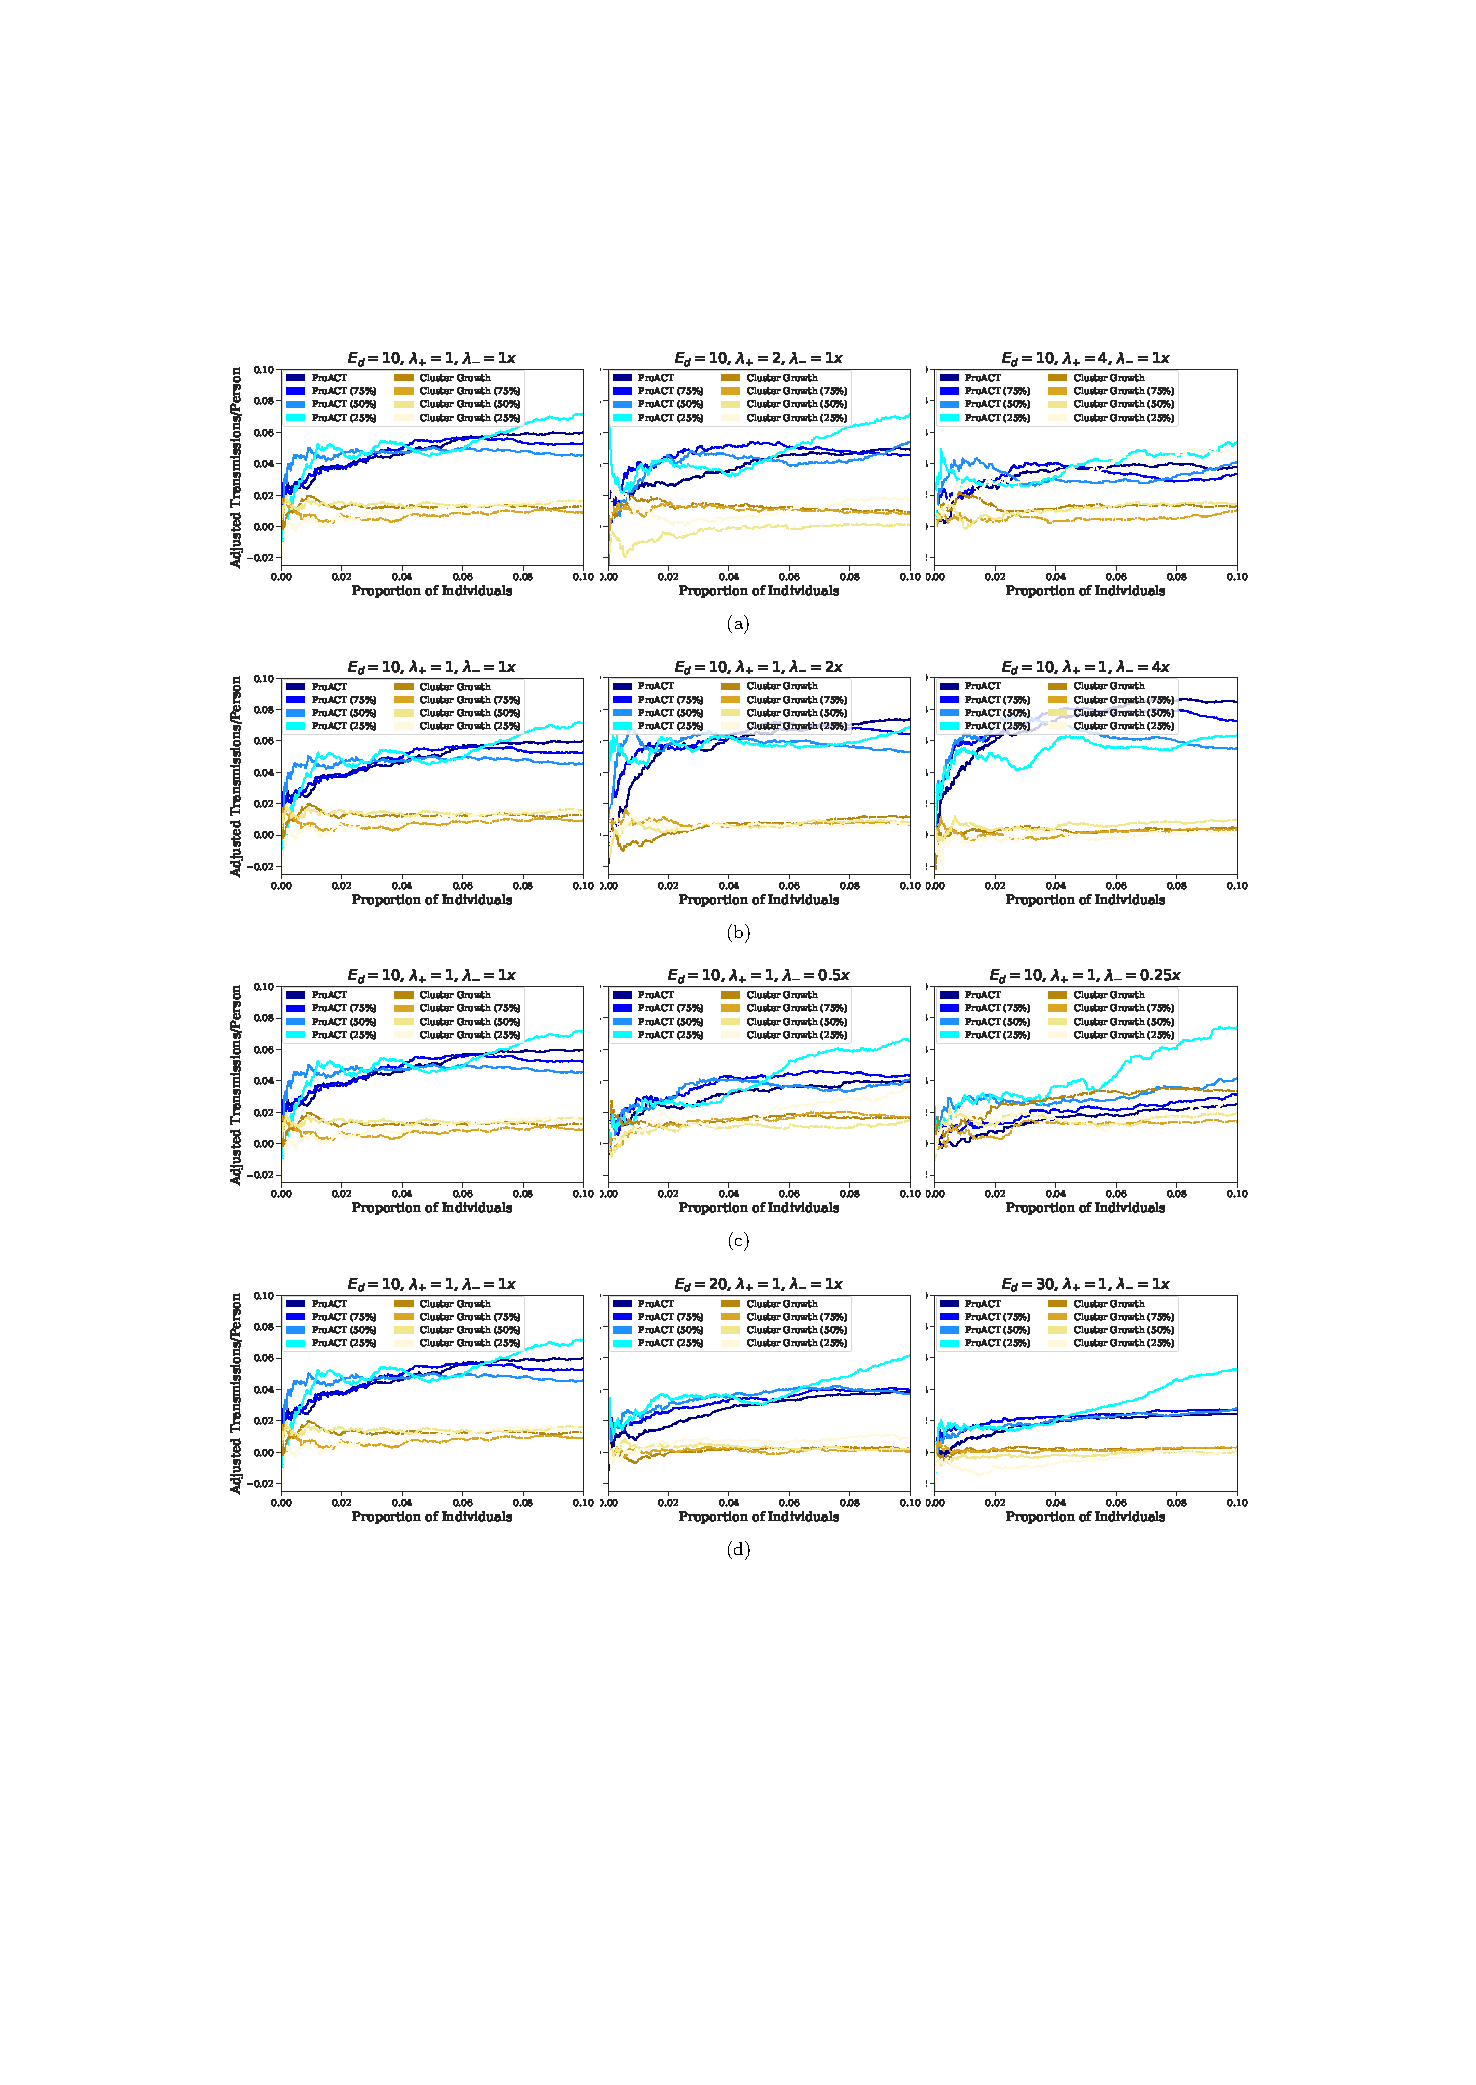
\includegraphics[width=0.77\textwidth]{figs/proact-efficacy}
\caption[Adjusted ProACT Performance on Simulated Datasets]
{ProACT performance on datasets simulated using FAVITES. \gls{CMA} of adjusted number of transmissions per person across the first decile of prioritized \glspl{PLWH} for each simulation parameter set. The horizontal axis depicts the quantile of highest-prioritized \glspl{PLWH} (e.g. $x=0.01$ denotes the top percentile), and the vertical axis depicts their adjusted average number of transmissions per person (1 indicates the optimal ordering, and 0 indicates an ordering that is no better than random). In our simulations, we varied three parameters of interest: (a) the rate of \gls{ART} initiation $(\lambda_+)$, (b-c) the rate of \gls{ART} termination $(\lambda_-)$, and (d) the expected degree of the sexual network $(E_d)$. The simulations were 10 years in length, prioritization was performed 9 years into the simulation, and the adjusted average number of transmissions per person was computed during the last year of the simulation. The curves labeled ``Cluster Growth'' denote prioritization by inferring transmission clusters using HIV-TRACE~\cite{Pond2018} at year 9 of the simulation and sorting clusters in descending order of growth rate since year 8. The curves labeled with percentages denote subsampled datasets. All curves were calculated using 20 simulation replicates.}
\label{fig:proact-efficacy}
\end{figure}

\subsubsection{ProACT Outperforms Random Prioritization Across Conditions}
Across all experimental parameters, ProACT performed much better than one would expect from a random ordering (Fig.~\ref{fig:proact-efficacy}). As we increased the proportion of top individuals selected, ProACT's \gls{CMA} initially increased (e.g. for up to 7\% top individuals in the base model condition) and subsequently flattened out. The most clear signal for benefits of prioritization (e.g, a high \gls{CMA}) is obtained for up to 10\% top-priority individuals (though exact values depend on the model condition).  As the number of selected individuals increases beyond 10\%, however, because the metric of efficacy is \gls{CMA}, the efficacy of a selection will eventually converge towards the efficacy of a random selection by definition (Fig.~\ref{fig:proact-efficacy-wide}).

\subsubsection{ProACT Outperforms Cluster Growth}
As mentioned, Wertheim \textit{et al}. (2018) present a method for prioritizing \glspl{PLWH} by clustering individuals based on viral genetic distance, tracking the size of each cluster over time, and prioritizing clusters in descending order of the growth rate~\cite{Wertheim2018}. The approach can be easily extended to also order individuals (i.e., individuals belonging to clusters with high growth rates are prioritized higher; see Materials and Methods for details). ProACT consistently outperformed prioritization using cluster growth for various parameter choices (Figs.~\ref{fig:proact-efficacy}--\ref{fig:proact-efficacy-vs-n}). The only exception was when the rate of stopping \gls{ART} was lowered all the way to 0.25x, which corresponds to expected time of \gls{ART} termination of 8.3 years. In this condition where adherence was at its highest, prioritization by cluster growth outperformed ProACT when using the full dataset.

\subsubsection{Impact of Simulation Parameters}
As the rate of stopping \gls{ART} $\left(\lambda_{-}\right)$ increased (i.e., with lower adherence), the gap between ProACT and cluster growth grows.
For example, the mean number of transmissions per person among the top 1,000 individuals chosen using ProACT and cluster growth were respectively 0.1702 and 0.0745 (a 1.28x improvement) for the condition with $\lambda_-=4$x. 
This 1.28x improvement gradually decreases to  0.95x, 0.78x, 0.31x, and -0.15x as we reduce the rate or ART termination to 2x, 1x, 0.5x, and 0.25x.
As  $\lambda_{-}$ decreased, ProACT's performance compared to optimal ordering tended to decrease, whereas cluster growth's performance compared to optimal ordering tended to increase; however, ProACT continued to outperform cluster growth for all but the $\lambda_-=$0.25X condition (Fig.~\ref{fig:proact-efficacy}b--c).

\begin{figure} % FIGURE 3 IN ORIGINAL PAPER
\centering
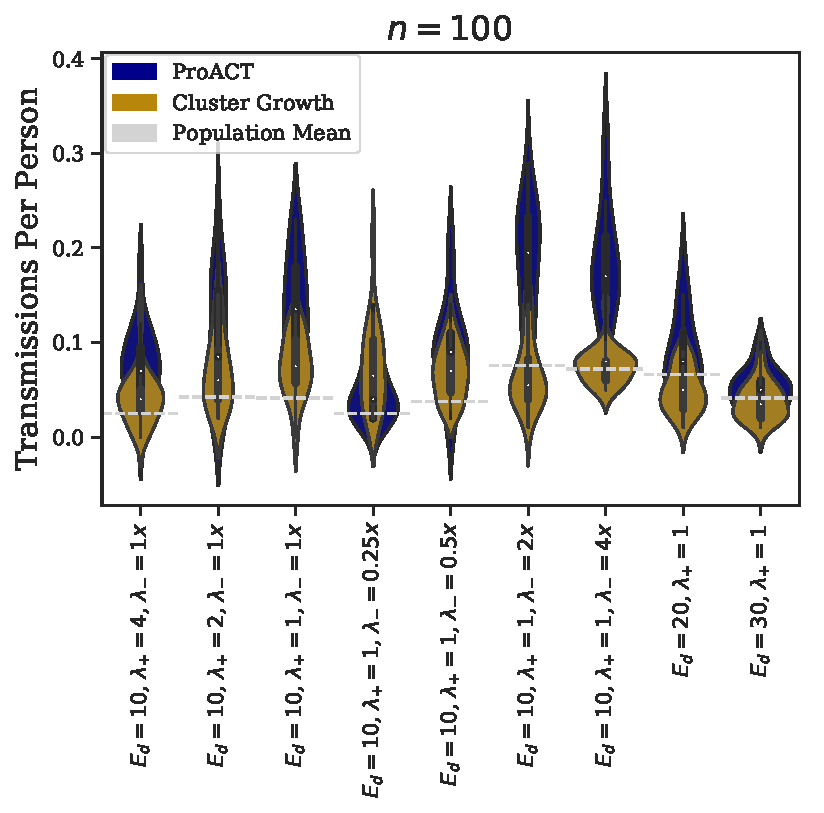
\includegraphics[width=0.495\textwidth]{figs/proact-efficacy-vs-n-100}
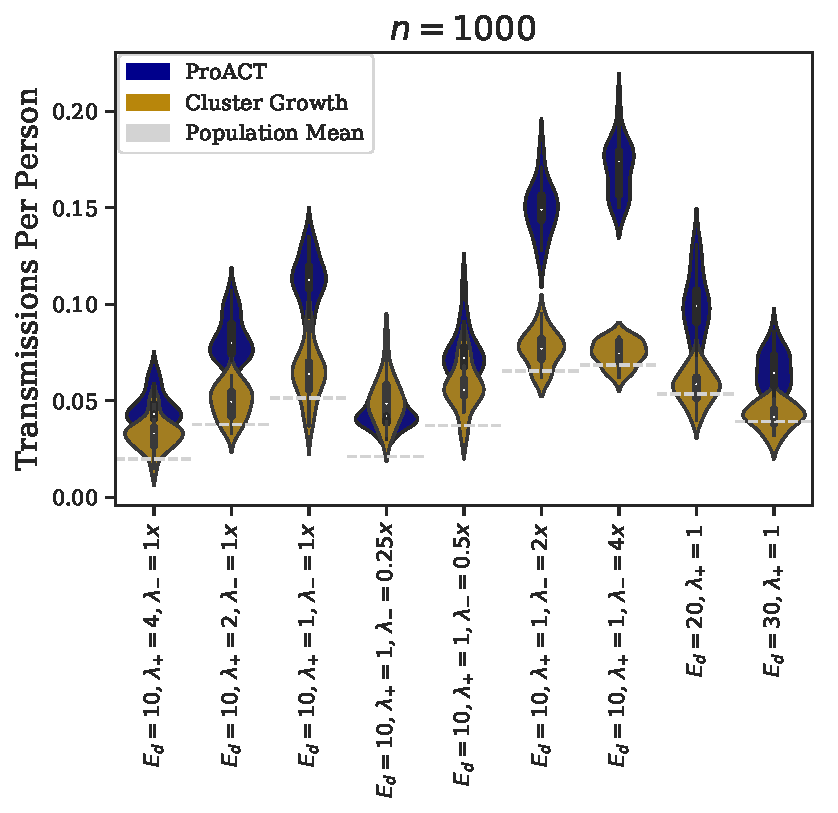
\includegraphics[width=0.495\textwidth]{figs/proact-efficacy-vs-n-1000}
\caption[Raw ProACT Performance vs. Number of Individuals]
{Efficacy on datasets simulated using FAVITES. Average of the raw number of transmissions per person for the top $n$ individuals in a prioritized list vs. simulation parameter set across various values of $n$. The violin plots depicted are across 20 replicates and contain box plots with distribution medians shown as white dots and distribution means shown as dashed grey lines.}
\label{fig:proact-efficacy-vs-n}
\end{figure}

As the rate of starting \gls{ART} $\left(\lambda_{+}\right)$ increased (i.e., with faster diagnoses), the performance of ProACT compared to optimal ordering very slightly degrades (Fig.~\ref{fig:proact-efficacy}a). As a result, the gap between ProACT and cluster growth decreases slightly: when observing the mean number of transmissions per person among the top 1,000 individuals chosen by each method, ProACT experiences a 0.78x, 0.70x, and 0.37x improvement over cluster growth when $\lambda_{+}$ is set to 1x, 2x, and 4x, respectively. Note that as expected, increasing $\lambda_{+}$ reduced the raw number of new infections caused per capita (Fig.~\ref{fig:proact-efficacy-raw}) overall and among top-priority individuals (Fig.~\ref{fig:proact-efficacy-vs-n}).

Effects of the expected number of sexual contacts per person $\left(E_d\right)$, which controls the speed of spread is also interesting (Figs.~\ref{fig:proact-efficacy}d and \ref{fig:proact-efficacy-vs-n}). As $E_d$ increased, the efficacy of both approaches decreased, but ProACT continued to consistently perform many times better than cluster growth.

\subsubsection{Impact of Incomplete Sampling}
Subsampling the total dataset to include $\sfrac{3}{4}$, $\sfrac{1}{2}$, or $\sfrac{1}{4}$ of the total population of \glspl{PLWH} did not have a major impact on the performance of ProACT compared to the optimal ordering (Fig.~\ref{fig:proact-efficacy}). Inevitably, the raw number of new infections decreased as the dataset was subsampled (Fig.~\ref{fig:proact-efficacy-raw}).  However, what remained relatively constant was the benefit of ProACT and cluster growth with respect to optimal and random ordering (e.g. the adjusted metric).

Despite the general robustness, some interesting effects were observed. With $\lambda_{+}=2$x, ProACT's performance remained quite similar across all levels of subsampling, whereas prioritization by cluster growth was negatively impacted by less sampling, especially at the $\sfrac{1}{4}$ level (Fig.~\ref{fig:proact-efficacy}a). Interestingly, for  $\lambda_{-}<1$x, ProACT's performance on  $\sfrac{1}{4}$ sampled datasets \textit{improved} relative to more complete sampling. However, the efficacy of prioritization by cluster growth remained fairly consistent  for  $\lambda_{-}<1$x (Fig.~\ref{fig:proact-efficacy}b--c). Similarly, the performance of ProACT compared to optimal ordering improved with $\sfrac{1}{4}$ sampled datasets when sexual contact degree increased to $E_d\geq 20$ (Fig.~\ref{fig:proact-efficacy}d).

\subsection{Real San Diego Dataset}
We next analyzed a dataset of 926 \gls{HIV}-1 subtype B \gls{pol} sequences obtained in San Diego between 1996 and 2018. To evaluate ProACT accuracy, we divided the data into deciles, with each decile defining two sets: \textit{past} (sequences up to the decile) and \textit{future} (sequences after the decile). We inferred a phylogeny from the sequences present in the \textit{past} set using FastTree~2~\cite{Price2010}, and we used ProACT to order all \glspl{PLWH} in this set. We then evaluated how the outcome measure correlates with the position of each individual in the ordering. We quantify the correlation using Kendall's tau-b, a rank correlation coefficient adjusted for ties~\cite{Kendall1938}. Values range between -1 and 1, with -1 signifying perfect inversion, 1 signifying perfect agreement, and 0 signifying the absence of association.

\begin{figure} % FIGURE 4 IN ORIGINAL PAPER
\centering
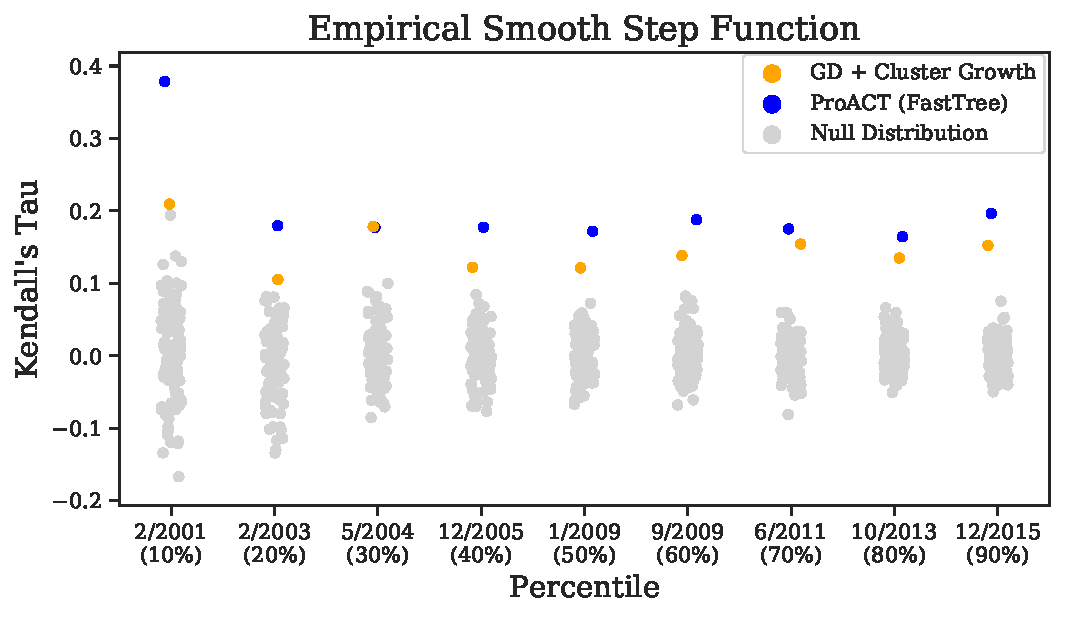
\includegraphics[width=0.495\textwidth]{figs/proact-tautest-smooth}
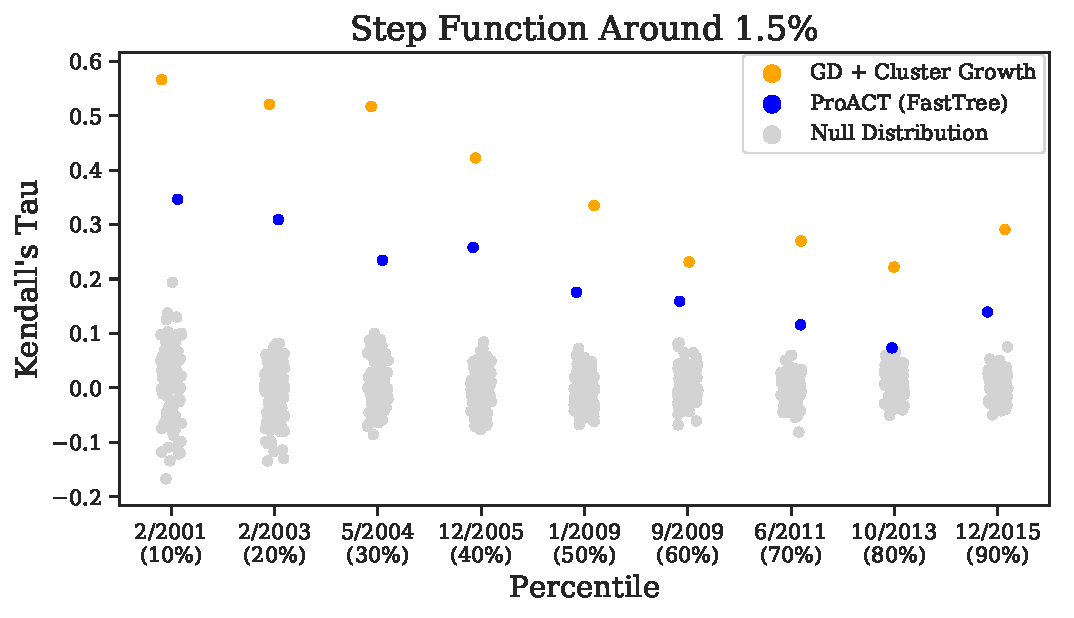
\includegraphics[width=0.495\textwidth]{figs/proact-tautest-strict}
\caption[Kendall's Tau-b Test \textit{p}-Values (Step Functions)]
{Kendall's tau-b test results for ProACT ordering on real data using two riskiness score functions: an empirical smooth step function and a strict step function around 1.5\%. The full San Diego dataset was split into two sets (\textit{pre} and \textit{post}) at each decile (shown on the horizontal axis). The individuals in \textit{pre} were ordered using ProACT and by cluster growth, and they were given a riskiness ``score'' computed using a riskiness score function (see Materials and Methods). Kendall's tau-b correlation coefficient was computed for each ordering with respect to the optimal possible ordering (i.e., sorting in descending order of riskiness score). The null distribution was visualized by randomly shuffling the individuals in \textit{pre}, and test \textit{p}-values are shown in Table~\ref{tab:proact-tautest}.}
\label{fig:proact-tautest}
\end{figure}

On real datasets, unlike the simulated data, the desired outcome measure, the number of new transmissions per person, is not known. Instead, we have to use inferred relationships. HIV-TRACE (used in our cluster growth approach) defines a pair of \glspl{PLWH} as ``genetically linked'' if their sequences are very similar (\gls{TN93} distance below 1.5\%). We similarly use the \gls{TN93} sequence similarity as an outcome measure, but in addition to using a fixed threshold, we also use smoother functions (Fig.~\ref{fig:proact-scorefuncs}). We measure the number of linked individuals using a step function (1 if \gls{TN93} distance is below 1.5\% and 0 otherwise) and an empirical smooth step function determined by fitting a mixture of three Gaussians to the distribution of pairwise \gls{TN93} distances (Material and Methods). We also explore an analytical smooth step function (parameterized sigmoid). Note that, when the step function is used, our outcome measure (computed for future transmissions) is exactly the same as what the cluster growth method uses for prioritizing (albeit, using past data). Thus, it is reasonable to expect the step function will favor cluster growth. As we move to smoother functions of distance to count genetic links, our measure is expected to become less biased in favor of HIV-TRACE.

\begin{table}[!ht] % TABLE 2 IN ORIGINAL PAPER
\caption[Kendall's Tau-b Test \textit{p}-Values (Step Functions)]{Kendall's tau-b test for a null hypothesis that a given prioritization yields a total outcome measure no better than random. We show \textit{p}-values for the real San Diego dataset for the first through ninth deciles using two outcome measure functions. Tests that failed to reject the null hypothesis with (uncorrected) \textit{p}-value $< 0.00138$ (corresponding to $\alpha=0.05$ with a Bonferroni multiple hypothesis testing correct with $n=36$) are marked with \dag.}
\vspace{-0.25in}
\begin{center}
Empirical Smooth Step Function\\
\begin{tabular}{|c|c|c|}
\hline
\textbf{Percentile} & \textbf{GD + Cluster Growth} & \textbf{ProACT (FastTree)}\\
\hline
10\% & $^\dag2\times10^{-3}$ & $^{\ }5\times10^{-8}$\\
\hline
20\% & $^\dag2\times10^{-2}$ & $^{\ }1\times10^{-4}$\\
\hline
30\% & $^{\ }5\times10^{-6}$ & $^{\ }6\times10^{-6}$\\
\hline
40\% & $^{\ }2\times10^{-4}$ & $^{\ }2\times10^{-7}$\\
\hline
50\% & $^{\ }5\times10^{-5}$ & $^{\ }2\times10^{-8}$\\
\hline
60\% & $^{\ }6\times10^{-7}$ & $^{\ }2\times10^{-11}$\\
\hline
70\% & $^{\ }2\times10^{-9}$ & $^{\ }1\times10^{-11}$\\
\hline
80\% & $^{\ }2\times10^{-8}$ & $^{\ }1\times10^{-11}$\\
\hline
90\% & $^{\ }2\times10^{-11}$ & $^{\ }1\times10^{-17}$\\
\hline
\end{tabular}
~\\~\\
Step Function Around 1.5\%\\
\begin{tabular}{|c|c|c|}
\hline
\textbf{Percentile} & \textbf{GD + Cluster Growth} & \textbf{ProACT (FastTree)}\\
\hline
10\% & $^{\ }4\times10^{-12}$ & $^{\ }1\times10^{-5}$\\
\hline
20\% & $^{\ }1\times10^{-19}$ & $^{\ }5\times10^{-8}$\\
\hline
30\% & $^{\ }3\times10^{-28}$ & $^{\ }3\times10^{-7}$\\
\hline
40\% & $^{\ }7\times10^{-25}$ & $^{\ }2\times10^{-10}$\\
\hline
50\% & $^{\ }2\times10^{-19}$ & $^{\ }1\times10^{-6}$\\
\hline
60\% & $^{\ }8\times10^{-12}$ & $^{\ }1\times10^{-6}$\\
\hline
70\% & $^{\ }1\times10^{-17}$ & $^{\ }1\times10^{-4}$\\
\hline
80\% & $^{\ }5\times10^{-14}$ & $^\dag7\times10^{-3}$\\
\hline
90\% & $^{\ }2\times10^{-25}$ & $^{\ }4\times10^{-7}$\\
\hline
\end{tabular}
\end{center}
\label{tab:proact-tautest}
\end{table}

Using both ProACT and cluster growth to prioritize individuals results in orderings of individuals with positive Kendall's tau-b correlations to the number of future genetic links  regardless of the time (i.e., decile) and the function used to count genetic links (Fig.~\ref{fig:proact-tautest}). These correlations are statistically significant in almost all cases  (Table~\ref{tab:proact-tautest} and Fig.~\ref{fig:proact-tautest}). The correlation coefficient ranges ranges between 0.4 (ProACT; 10\% time) and 0.1 (cluster growth; 20\% time) for empirical function, and between 0.6 (cluster growth; 10\% time) and 0.1 (ProACT; 80\% time) for the step function.

The comparison between ProACT and cluster growth depends on the choice of the function to count links. When counting the number of links using the step function, prioritization by cluster growth consistently outperforms ProACT for all deciles of the dataset. These results are not surprising, given that we count HIV-TRACE links both to prioritize and to evaluate. However, according to the empirical smooth step function learned from the \gls{TN93} distances, ProACT outperforms cluster growth in all except one time point, where they are tied.

To further test whether the smoothness of the link-counting function applied to \gls{TN93} distances is a factor in deciding the relative accuracy of methods, we used a sigmoid function to replace the step function while keeping the inflection point at 1.5\% (Fig.~\ref{fig:proact-scorefuncs}). We observed that as the outcome measure function becomes more smooth, ProACT's performance improves with respect to prioritization by cluster growth (Fig.~\ref{fig:proact-tautest-sup}, Table~\ref{tab:proact-tautest-sup}). Based on the more smooth sigmoid function ($\lambda=5$), ProACT outperforms cluster growth in all but one case where they are tied. Thus, simply counting distances close to 1.5\% as partial links leads to evaluations that favor ProACT.

\begin{figure} % FIGURE 5 IN ORIGINAL PAPER
\centering
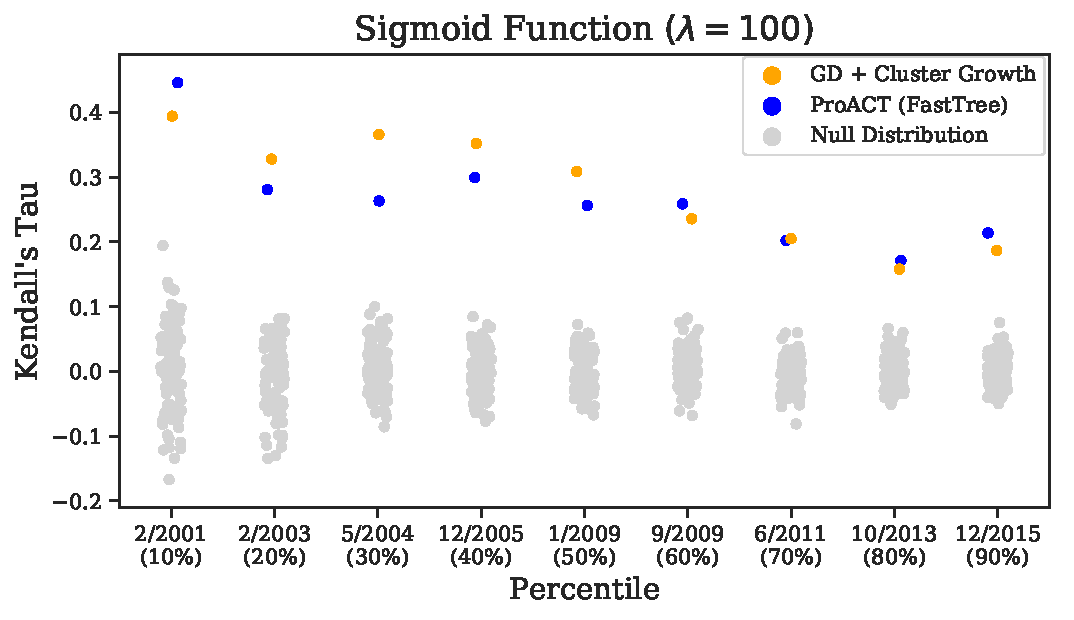
\includegraphics[width=0.495\textwidth]{figs/proact-tautest-L100}
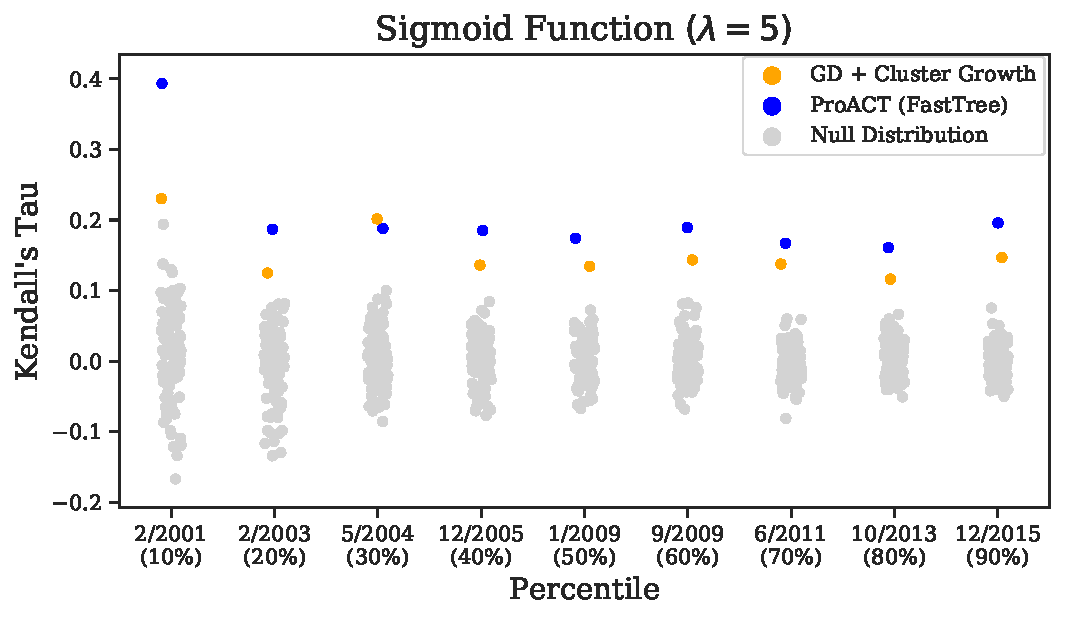
\includegraphics[width=0.495\textwidth]{figs/proact-tautest-L5}
\caption[Kendall's Tau-b Test \textit{p}-Values (Sigmoid Functions)]
{Kendall's tau-b test results for ProACT ordering on real data using the sigmoid riskiness score functions with $\lambda=100$ and $\lambda=5$. The full San Diego dataset was split into two sets (\textit{pre} and \textit{post}) at each decile (shown on the horizontal axis). The individuals in \textit{pre} were ordered using ProACT and by cluster growth, and they were given a riskiness ``score'' computed using a riskiness score function (see Materials and Methods). Kendall's tau-b correlation coefficient was computed for each ordering with respect to the optimal possible ordering (i.e., sorting in descending order of riskiness score). The null distribution was visualized by randomly shuffling the individuals in \textit{pre}, and test \textit{p}-values are shown in Table~\ref{tab:proact-tautest-sup}.}
\label{fig:proact-tautest-sup}
\end{figure}

As time increases, both methods experience seemingly downward trends in their tau coefficients, but the null distribution of tau coefficients also tightens  (Fig.~\ref{fig:proact-tautest}). Thus, both methods consistently do significantly better than expected by random chance and there is no clear relationship between \textit{p}-values of individual tool and time (Table~\ref{tab:proact-tautest}). However, both for the step function and the sigmoid functions, ProACT's relative performance with respect to cluster growth tends to improved over time.

\section{Discussion}
We start by discussing observed results and then comment on practical implications of this paper both for public health and for future research in molecular epidemics. 

\subsection{Discussion of Results}
In our simulations, ProACT was least effective in conditions with very low rate of \gls{ART} termination $(\lambda_{-})$ which correspond to very high adherence. As expected, the total number of new infections originated from \glspl{PLWH} is low when adherence is high (Fig.~\ref{fig:proact-efficacy-raw}) and neither method is much better than random clustering. This observation is consistent with the motivation we presented for the ProACT algorithm. Recall that the motivation relied on identifying \glspl{PLWH} who have stopped being suppressed. If all known \glspl{PLWH} have been started on treatment and none ever stops treatment, prioritization loses its practical relevance, and relatedly, ProACT loses its statistical power. We saw a similar effects when we increased the rate of \gls{ART} $(\lambda_{+})$, which is also not surprising as increasing $\lambda_{+}$ is in effect similar to reducing $\lambda_{-}$.

When we reduced sampling, we did not observe reductions in effectiveness of ProACT and occasionally even observed improvements. These results have to be interpreted in the context of our adjusted metric, which measures benefits over random and below optimal ordering. The per capita number of new infections from high-priority \glspl{PLWH} was \textit{lowered} when we subsampled the datasets (Fig.~\ref{fig:proact-efficacy-raw}). Thus, as expected, when some \glspl{PLWH} are missing from the dataset available to a particular analysis, the overall effectiveness of identifying top priority \glspl{PLWH} reduces. However, the effectiveness reduces equally for the optimal ordering and the ProACT method is not impacted any worse than optimal ordering is. In fact, ProACT is in some cases impacted a bit less harshly than optimal ordering, hence the improvements in adjusted outcome with $\sfrac{1}{4}$ sampling. One should also keep in mind that choosing $x$\% highest priority individuals from the full datasets results in 4x as many individuals as choosing the top $x$\% of the $\sfrac{1}{4}$ subsampled dataset.

The reader is reminded that \glspl{PLWH} are \glspl{PLH} who are also diagnosed, and in our model, are immediately sequenced and put on \gls{ART} (which they may or may not sustain). Thus, \textit{full sampling} refers to a case where all \textit{diagnosed} individuals are included in the dataset and \glspl{PLH} who are not diagnosed are never in our sampling. In other words, the full sampling case should not be misunderstood as including undiagnosed people. Rather, lack of full sampling corresponds to a case where some \glspl{PLWH} are known to \textit{some} clinic but are not included in the study, perhaps due to a lack of sequencing or data sharing.

ProACT far outperformed random ordering and also ordering by cluster growth in simulations. However, we note that, despite the strong performance, there is much room left for future improvement: ProACT consistently ranges in its outcome measure between 2\% and 10\% of the theoretically optimal efficacy when selecting up to 10\% of top-priority \glspl{PLWH}. Thus, there is great room for improvement in identifying high-value individuals compared to our method according to the simulation results. It will be unrealistic to expect that any statistical method based solely on sequence data (and perhaps also commonly available metadata, e.g. sampling times) will be able to come close to the optimal ordering. Nevertheless, it remains likely that methods better than ProACT could in fact be developed.

\subsection{Implications of Results}
In this paper, in addition to introducing ProACT, we formalized a useful approach for thinking about the effectiveness of public health intervention in molecular epidemics. Instead of focusing on the accuracy of methods of reconstructing phylogenetic trees or transmission networks, a question fraught with difficulties, we asked a more practical question. Given molecular epidemic data, can the methods, whether phylogenetic or clustering-based, prioritize \glspl{PLWH} for increased attention by public health? The idea of using molecular epidemics for prioritization is of course not a new idea. For example, as we mentioned, Wertheim \textit{et al}. (2018) presented a method to prioritize \glspl{PLWH} based on the growth rates of their transmission clusters~\cite{Wertheim2018}. Vasylyeva \textit{et al}. (2018) performed a phylogeographic analysis to reconstruct \gls{HIV} movement among different locations in Ukraine in order to infer region-level risk prioritization~\cite{Vasylyeva2018}. Much earlier even, Mellors \textit{et al}. (1996) predicted \gls{HIV} patient prognosis by quantifying \gls{HIV} \gls{RNA} in plasma~\cite{Mellors1996}; predicted prognosis can subsequently be used as a prioritization rank. However, we hope that our formal definition of the problem as a computational question (i.e., prioritization), in addition to our extensive simulations and developed metrics of evaluation will stir further work in this area. As stated before, it seems likely that more advanced methods than our simple prioritization approach can improve performance beyond ProACT in the future.

ProACT prioritizes individuals, not clusters. Prioritizing treatment followup or partner tracing for individuals based on their perceived risk of future transmission promises to be perhaps more effective than targeting clusters. However, such targeted approaches also pose ethical questions that have to be considered. For example, we may not want the algorithm to be biased towards particular demographic attributes. ProACT does not use \textit{any} metadata in its prioritization, reducing risks of such biases. It simply uses the viral phylogeny, which, compared to other types of data, may lead to fewer biases. Nevertheless, it is possible that factors such as the depth of the sampling of a demographic group can in fact change branch length patterns in the phylogeny and make ProACT less or more effective for certain demographic groups. These broader implications of individual prioritization and impacts of demographics on the performance of ProACT should be studied more carefully in future.

One may wonder whether ordering by branch lengths will result in orderings that fail to change with time and reflect the changes in the epidemic. To answer this question, on the San Diego \gls{PIRC} data, we asked how fast the ProACT ordering changes as time progresses. To do so, we computed Kendall's tau-b correlations to the ProACT ordering obtained using only the first decile of the dataset (Fig.~\ref{fig:proact-tautest-first-proact}). There was a strong but diminishing correlation with the initial ordering. The correlations started at 1 (as expected) and gradually decreased in the ninth decile to 0.522. The results show that as desired, ProACT orders do in fact change with time, albeit gradually. The gradual change implies that certain individuals remain high-priority as time progresses. In practical use, ProACT ordering should be combined with clinical knowledge about the status of individual patients. For example, high priority individuals according to ProACT can be given lower priority if they manage to constantly remain suppressed with multiple followups. More broadly, the ProACT ordering should be considered one more tool for prioritizing clinical care, but valuable clinical knowledge, not incorporated into the algorithm, should also be exploited.

Finally, a question faced by public health officials is whether the cost of targeting diagnosed individuals for followups and partner tracing is worth the reduction in future cases. The answer to that question will inevitably depend on who is targeted. For example, in our default simulation case, targeting individuals randomly would at most reduce 0.0529 transmissions per chosen person in the next 12 months, whereas targeting top 1000 individuals according to ProACT would at most reduce 0.119 transmissions. Thus, prioritization can in fact change the cost-benefit analyses. Moreover, given a prioritization, one can use simulations to predict the outcome measure for the top $x$ individuals (similar to Fig.~\ref{fig:proact-efficacy}) and use metrics such as \gls{QALY} to estimate how many top individuals should be targeted for the cost to justify the benefits.

\section{Materials and Methods}
\subsection{Simulated Datasets}
We used FAVITES to simulate a sexual contact network, transmission network, viral phylogeny, and viral sequences emulating \gls{HIV} transmission in San Diego from 2005 to 2014~\cite{Moshiri2018}.

Transmissions were modeled using a compartmental epidemiological model with 5 states: Susceptible (S), Acute \gls{HIV} Untreated (AU), Acute \gls{HIV} Treated (AT), Chronic \gls{HIV} Untreated (CU), and Chronic \gls{HIV} Treated (CT). Individuals in state S (i.e., uninfected) can only transition to state AU. Each infected state $x\in\{\text{AU},\text{AT},\text{CU},\text{CT}\}$ defines a ``rate of infectiousness'' $\lambda_{\text{S},x}$: given an uninfected individual $u$ in state S who has $n_x$ sexual partners in state $x\in\{\text{AU},\text{AT},\text{CU},\text{CT}\}$, the transition of $u$ from S to AU is a Poisson process with rate $\lambda_u=\sum_{x\in\{\text{AU},\text{AT},\text{CU},\text{CT}\}}{n_{x}\lambda_{\text{S},x}}$. To mimic reality, where ART significantly reduces the risk of transmission, rates are chosen such that $\lambda_{\text{S},\text{AU}} > \lambda_{\text{S},\text{CU}} > \lambda_{\text{S},\text{AT}} > \lambda_{\text{S},\text{CT}} \approx 0$. At the beginning of the epidemic simulation, all initially uninfected individuals are placed in state S, and all initially infected (i.e., ``seed'') individuals are distributed among the 4 infected states according to their steady-state proportions. This model is a simplified version of the model proposed by Granich \textit{et al}. (2009)~\cite{Granich2009}.

For the most part, we used the base parameters used in Moshiri \textit{et al}. (2018) that sought to model San Diego~\cite{Moshiri2018}, with the following modifications to better capture reality. See Table~\ref{tab:proact-config-file} for the full set of parameters of the default condition.

\paragraph{Sexual Contact Network.} To capture the scale-free nature of the sexual contact network, Moshiri \textit{et al}. (2018) used the \gls{BA} model~\cite{Barabasi1999}. In addition to the scale-free property, in \gls{HIV} sexual networks, we typically observe many densely-connected communities~\cite{Rothenberg1998}, a property the \gls{BA} model fails to directly model. To have control over the number of communities,  we simulated sexual contact networks such that networks contained 20 \gls{BA} communities, each with 5,000 individuals. In the base condition, the expected degree of connection between an individual and somebody \textit{within} their community was chosen to be 10, and the expected degree between an individual and somebody \textit{outside} their community was chosen to be 1. Each community was simulated separately using the \gls{BA} model and connections between communities were chosen uniformly at random, akin to the \gls{ER} model~\cite{Erdos1959}. Estimates from the literature put the number of contacts at 3--4 during a single year~\cite{Rosenberg2011}. Because our simulated sexual contacts remain static over the 10 year simulation period, we explore mean degrees between 10 and 30.

\paragraph{Epidemic Initialization.} In Moshiri \textit{et al}. (2018), at the start of the epidemic, all infected individuals were in state AU~\cite{Moshiri2018}. Here, instead, we randomly distribute initially infected individuals according to expected proportions of the states. To find these proportions, we ran simulations in which all seed individuals were in state AU, and we observed the proportion of individuals in each state over time, which reached a steady-state fairly early in the simulations (Fig.~\ref{fig:proact-prop-state-vs-time}).

\paragraph{Time of Sequencing.} In Moshiri \textit{et al}. (2018), viral sequences are obtained from individuals exactly at the end time of the 10-year simulation period~\cite{Moshiri2018}. In reality, however, \gls{HIV} patients are typically sequenced when they first visit a clinic to receive \gls{ART}. Thus, it is expected that the terminal branch lengths of trees simulated in Moshiri \textit{et al}. (2018) are artificially longer than would be expected. Instead, we sample viral sequences from individuals the first time they begin \gls{ART} (i.e., the first time they enter state AT or CT). Our current simulation better captures standards of care in advanced health care systems.

\subsubsection{Simulated Data Analysis}
For each simulated sequence dataset, using FastTree~2~\cite{Price2010}, a phylogenetic tree was inferred under the \gls{GTR}+$\Gamma$ model from the sequences obtained in the first 9 years of the simulation. These trees were then MinVar-rooted using FastRoot~\cite{Mai2017}, and ProACT was run on the resulting trees.

\subsection{San Diego Dataset}
To test ProACT on real data, we used a \gls{MSA} of 926 \gls{HIV}-1 subtype B \gls{pol} sequences from San Diego collected by the UC San Diego \gls{PIRC}. \gls{PIRC} is one of the largest longitudinal cohorts of \glspl{PLWH} in the United States. By design, \gls{PIRC} strives to include acute infections (as much as 40\% of recruited individuals are during acute or early stages of infection). Access to the data was obtained through a proposal submitted to \gls{PIRC}.

A phylogenetic tree was inferred from the \gls{MSA} under the \gls{GTR}+$\Gamma$ model using FastTree~2~\cite{Price2010}, and the resulting tree was MinVar-rooted using FastRoot~\cite{Mai2017}. For each decile, using TreeSwift~\cite{Moshiri2018b}, the full tree was pruned to only contain samples obtained up to the end of that decile. ProACT was run on each of the resulting trees.

\subsection{Evaluation Procedure}
\subsubsection{Simulated Data}
To measure the efficacy of a given ProACT selection, because the true transmission histories are known in simulation, we simply average the number of infections caused by the individuals in the selection in the last year of simulation (i.e, after prioritization) to obtain a raw outcome measure.

Let $A=\{1,\ldots,n\}$ denote the first, \ldots, $n$-th sampled individual in the current time step (years 1--9 in our simulations). For each individual $i$, let $c(i)$ denote the number of individuals directly infected by $i$ in the next time step (year 10 in our simulations). Given any set of individuals $s\subseteq A$, let $C(s)=\frac{1}{|s|}\sum_{i\in s}{c(i)}$ denote the average $c(i)$ for all individuals $i\in s$.

Let $x=(x_1,\ldots,x_n)$ denote an ordering of $A$. The (unadjusted) \gls{CMA} of $x$ up to $i$ is $C\left(\{x_1,\ldots,x_i\}\right)$. Let $o=(o_1,\ldots,o_n)$ denote the ordering of $A$ in which elements are sorted in descending order of $c(i)$ (i.e., the optimal ordering), with ties broken arbitrarily. We defined the adjusted \gls{CMA} of $x$ up to $i$ as
\begin{equation}\label{eq:cma}
    \frac{C\left(\{x_1,\ldots,x_i\}\right)-C(A)}{C\left(\{o_1,\ldots,o_i\}\right)-C(A)}\; .
\end{equation}
We use Equation~\ref{eq:cma} to measure the effectiveness of a selection of the top $i$ individuals from each ordering of all individuals. We explore $i$ for 1 to 10\% of the total number of samples (i.e., $\frac{|A|}{10}$).

\subsubsection{Real Data}
The sequences were sorted in ascending order of sample time and, for each decile, they were split at the decile to form two sets: \textit{pre} and \textit{post}. A phylogenetic tree was inferred from the sequences in \textit{pre} under the \gls{GTR}+$\Gamma$ model using FastTree~2~\cite{Price2010} and MinVar-rooted~\cite{Mai2017}. Using the resulting tree, ProACT ordered the samples. Then, pairwise distances were computed between each sequence in \textit{pre} and each sequence in \textit{post} under the \gls{TN93} model~\cite{Tamura1993} using the \texttt{tn93} tool of HIV-TRACE~\cite{Pond2018}.

A natural function to compute the riskiness score of a given individual $u$ in \textit{pre}, similar to that proposed by Wertheim \textit{et al}. (2018)~\cite{Wertheim2018}, is to simply count the number of individuals in \textit{post} who are genetic links to $u$, i.e., $\sum_{v\in post}{\left[d(u,v)\le1.5\%\right]}$. In other words, the score function is simply a step function with value 1 for all distances less than or equal to 1.5\% and 0 for all other distances. However, the selection of 1.5\% as the distance threshold, despite being common practice in many \gls{HIV} transmission clustering analyses, is somewhat arbitrary, and a step function exactly at this threshold may be overly strict (e.g. should a pairwise distance of 1.51\% be ignored?).

To generalize this notion of scoring links, we utilized three analytical score functions. The first is the aforementioned step function $f_1(d)=\left[d\le1.5\%\right]$. The second is a sigmoid function $f_2(d)=\frac{\lambda+1}{\lambda^{d/0.15}+\lambda}$ with the choice of $\lambda=100$ and $\lambda=5$ (Fig.~\ref{fig:proact-scorefuncs}). The third is an empirical scoring function learnt from the data by fitting a mixture model of three Gaussian random variables onto the distribution of pairwise \gls{TN93} distances $f_3(d)=\frac{p_1(x)}{p_1(x)+p_2(x)+p_3(x)}$, where $p_1(x)$ is the \gls{PDF} of the Gaussian component with smallest mean and $p_2(x)$ and $p_3(x)$ are the remaining Gaussian components (Fig.~\ref{fig:proact-scorefuncs}). Specifically, the three Gaussian fits were parameterized by ($\mu_1=0.0191$, $\sigma_1=0.0103$), ($\mu_2=0.0609$, $\sigma_2=0.0118$), and ($\mu_3=0.118$, $\sigma_3=0.0468$), respectively.

For each of these function, for each decile to define \textit{pre} and \textit{post}, we performed a Kendall's tau-b test to compare the prioritization approaches~\cite{Kendall1938}. To generate a null distribution in Figure~\ref{fig:proact-tautest}, we randomly shuffled the individuals in \textit{pre} repeatedly; note however that the \textit{p}-values reported in Table~\ref{tab:proact-tautest} are the theoretical \textit{p}-values computed by the tau-b test, not empirically estimated from our repeated shuffling.

\section{Acknowledgments}
We thank Susan B. Little for providing the San Diego \gls{HIV} sequence dataset used in this study. We also thank Joel O. Wertheim and Sanjay R. Mehta for fruitful discussions that helped motivate the development of ProACT.

This work was supported by the National Institutes of Health (5P30AI027767-28, AI100665, AI106039, and MH100974) and a developmental grant from the University of California, San Diego Center for AIDS Research (P30 AI036214), supported by the National Institutes of Health.

%% END PROACT CHAPTER